\begingroup
\definecolor{slitplus}{HTML}{28628A}
\definecolor{slitminus}{HTML}{B34E37}
\definecolor{slitink}{HTML}{313A43}
\definecolor{slitplug}{HTML}{DDE1E4}
\definecolor{slitcollar}{HTML}{EAF2EF}
\resizebox{0.98\linewidth}{!}{%
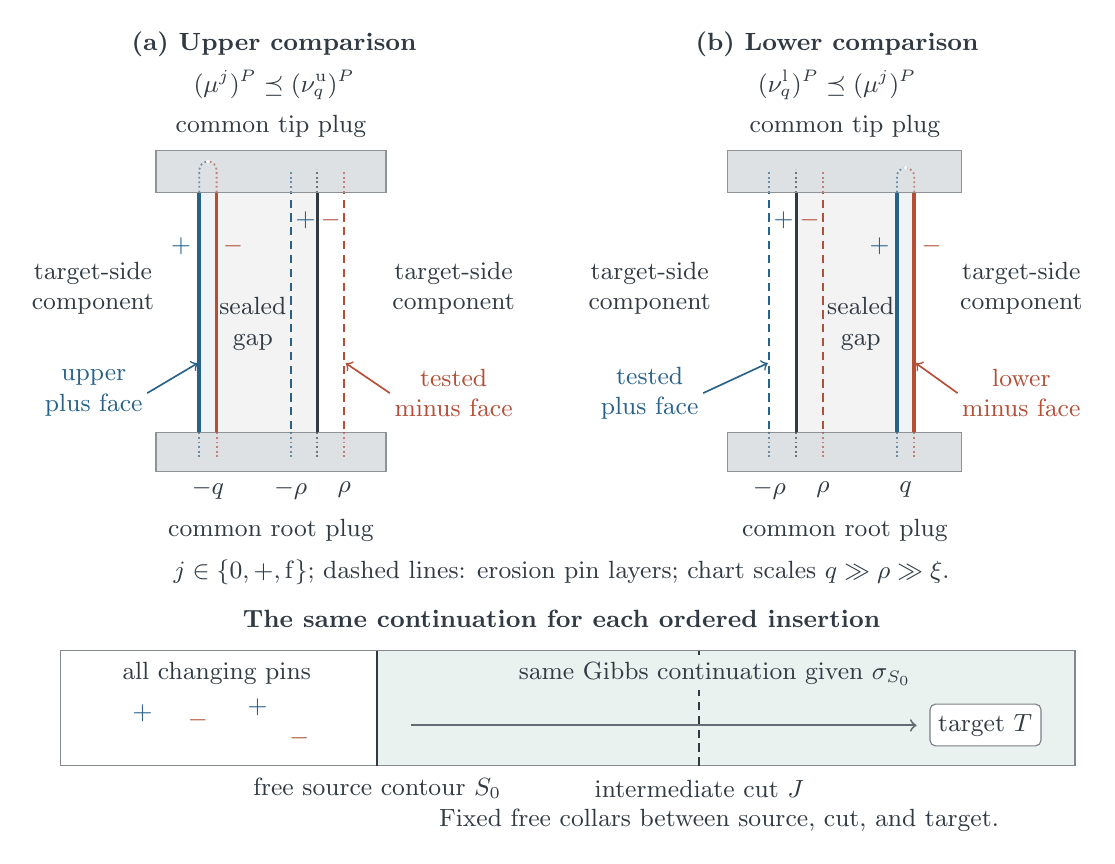
\begin{tikzpicture}[
  x=1cm,y=1cm,font=\small,text=slitink,
  wall/.style={draw=slitink,line width=1.15pt},
  plusface/.style={draw=slitplus,line width=1.35pt},
  minusface/.style={draw=slitminus,line width=1.35pt},
  pluslayer/.style={draw=slitplus,densely dashed,line width=.8pt},
  minuslayer/.style={draw=slitminus,densely dashed,line width=.8pt},
  plug/.style={fill=slitplug,draw=slitink!55,line width=.45pt},
  guide/.style={draw=slitink!60,line width=.45pt},
  ghost/.style={densely dotted,line width=.65pt,opacity=.65},
  every node/.style={inner sep=1.5pt,align=center}
]

\begin{scope}
  \node at (2.85,5.68) {\textbf{(a) Upper comparison}};
  \node at (2.85,5.16)
    {$(\mu^j)^P\preceq(\nu_q^{\mathrm u})^P$};

  \fill[slitink!6] (2.12,.60) rectangle (3.40,3.88);
  \node at (2.58,2.13) {sealed\\gap};
  \fill[slitplus!7] (1.90,.44) rectangle (2.12,4.04);
  \draw[plusface] (1.90,.44)--(1.90,4.04);
  \draw[minusface] (2.12,.44)--(2.12,4.04);
  \draw[wall] (3.40,.44)--(3.40,4.09);
  \draw[pluslayer] (3.06,.44)--(3.06,4.08);
  \draw[minuslayer] (3.74,.44)--(3.74,4.08);

  \node[text=slitplus] at (1.67,3.12) {$+$};
  \node[text=slitminus] at (2.33,3.12) {$-$};
  \node[text=slitplus] at (3.25,3.45) {$+$};
  \node[text=slitminus] at (3.57,3.45) {$-$};
  \node at (.55,2.58) {target-side\\component};
  \node at (5.13,2.58) {target-side\\component};

  \node[text=slitplus] (uplus) at (.56,1.25) {upper\\plus face};
  \draw[->,draw=slitplus,line width=.6pt]
    (uplus.east)--(1.88,1.63);
  \node[text=slitminus] (uminus) at (5.13,1.25) {tested\\minus face};
  \draw[->,draw=slitminus,line width=.6pt]
    (uminus.west)--(3.76,1.63);

  \draw[plug] (1.35,.25) rectangle (4.27,.75);
  \draw[plug] (1.35,3.80) rectangle (4.27,4.33);
  \node at (2.81,4.64) {common tip plug};
  \node at (2.81,-.49) {common root plug};
  \draw[ghost,draw=slitplus] (1.90,3.80)--(1.90,4.08)
    arc[start angle=180,end angle=90,radius=.11];
  \draw[ghost,draw=slitminus] (2.12,3.80)--(2.12,4.08)
    arc[start angle=0,end angle=90,radius=.11];
  \fill[white] (2.01,4.19) circle[radius=.025];
  \draw[ghost,draw=slitink] (3.40,3.80)--(3.40,4.09);
  \draw[ghost,draw=slitplus] (3.06,3.80)--(3.06,4.08);
  \draw[ghost,draw=slitminus] (3.74,3.80)--(3.74,4.08);
  \draw[ghost,draw=slitplus] (1.90,.75)--(1.90,.44);
  \draw[ghost,draw=slitminus] (2.12,.75)--(2.12,.44);
  \draw[ghost,draw=slitink] (3.40,.75)--(3.40,.44);
  \draw[ghost,draw=slitplus] (3.06,.75)--(3.06,.44);
  \draw[ghost,draw=slitminus] (3.74,.75)--(3.74,.44);

  \node at (2.01,.02) {$-q$};
  \node at (3.06,.02) {$-\rho$};
  \node at (3.74,.02) {$\rho$};
\end{scope}

\begin{scope}[shift={(7.10,0)}]
  \node at (2.90,5.68) {\textbf{(b) Lower comparison}};
  \node at (2.90,5.16)
    {$(\nu_q^{\mathrm l})^P\preceq(\mu^j)^P$};

  \fill[slitink!6] (2.38,.60) rectangle (3.66,3.88);
  \node at (3.20,2.13) {sealed\\gap};
  \fill[slitplus!7] (3.66,.44) rectangle (3.88,4.00);
  \draw[plusface] (3.66,.44)--(3.66,4.00);
  \draw[minusface] (3.88,.44)--(3.88,4.00);
  \draw[wall] (2.38,.44)--(2.38,4.09);
  \draw[pluslayer] (2.04,.44)--(2.04,4.08);
  \draw[minuslayer] (2.72,.44)--(2.72,4.08);

  \node[text=slitplus] at (3.44,3.12) {$+$};
  \node[text=slitminus] at (4.10,3.12) {$-$};
  \node[text=slitplus] at (2.22,3.45) {$+$};
  \node[text=slitminus] at (2.55,3.45) {$-$};
  \node at (.52,2.58) {target-side\\component};
  \node at (5.24,2.58) {target-side\\component};

  \node[text=slitplus] (lplus) at (.52,1.25) {tested\\plus face};
  \draw[->,draw=slitplus,line width=.6pt]
    (lplus.east)--(2.02,1.63);
  \node[text=slitminus] (lminus) at (5.24,1.25) {lower\\minus face};
  \draw[->,draw=slitminus,line width=.6pt]
    (lminus.west)--(3.90,1.63);

  \draw[plug] (1.51,.25) rectangle (4.48,.75);
  \draw[plug] (1.51,3.80) rectangle (4.48,4.33);
  \node at (3.00,4.64) {common tip plug};
  \node at (3.00,-.49) {common root plug};
  \draw[ghost,draw=slitplus] (3.66,3.80)--(3.66,4.00)
    arc[start angle=180,end angle=90,radius=.11];
  \draw[ghost,draw=slitminus] (3.88,3.80)--(3.88,4.00)
    arc[start angle=0,end angle=90,radius=.11];
  \fill[white] (3.77,4.11) circle[radius=.025];
  \draw[ghost,draw=slitink] (2.38,3.80)--(2.38,4.09);
  \draw[ghost,draw=slitplus] (2.04,3.80)--(2.04,4.08);
  \draw[ghost,draw=slitminus] (2.72,3.80)--(2.72,4.08);
  \draw[ghost,draw=slitplus] (3.66,.75)--(3.66,.44);
  \draw[ghost,draw=slitminus] (3.88,.75)--(3.88,.44);
  \draw[ghost,draw=slitink] (2.38,.75)--(2.38,.44);
  \draw[ghost,draw=slitplus] (2.04,.75)--(2.04,.44);
  \draw[ghost,draw=slitminus] (2.72,.75)--(2.72,.44);

  \node at (2.04,.02) {$-\rho$};
  \node at (2.72,.02) {$\rho$};
  \node at (3.77,.02) {$q$};
\end{scope}

\node at (6.50,-1.02)
  {$j\in\{0,+,\mathrm f\}$; dashed lines: erosion pin layers;
   chart scales $q\gg\rho\gg\xi$.};

\node at (6.50,-1.62) {\textbf{The same continuation for each ordered insertion}};
\fill[slitcollar] (4.16,-3.48) rectangle (13.02,-2.02);
\draw[guide] (.14,-3.48) rectangle (13.02,-2.02);
\node at (2.12,-2.31) {all changing pins};
\node[text=slitplus] at (1.18,-2.82) {$+$};
\node[text=slitminus] at (1.88,-2.91) {$-$};
\node[text=slitplus] at (2.64,-2.74) {$+$};
\node[text=slitminus] at (3.17,-3.13) {$-$};
\draw[draw=slitink,line width=.8pt] (4.16,-3.48)--(4.16,-2.02);
\draw[draw=slitink,densely dashed,line width=.8pt]
  (8.25,-3.48)--(8.25,-2.02);
\node[fill=slitcollar] at (8.45,-2.32)
  {same Gibbs continuation given $\sigma_{S_0}$};
\draw[->,draw=slitink!75,line width=.7pt] (4.59,-2.97)--(11.01,-2.97);
\draw[rounded corners=2pt,fill=white,draw=slitink!65]
  (11.18,-3.23) rectangle (12.59,-2.70);
\node at (11.88,-2.965) {target $T$};
\node at (4.16,-3.77) {free source contour $S_0$};
\node at (8.25,-3.77) {intermediate cut $J$};
\node at (8.50,-4.18)
  {Fixed free collars between source, cut, and target.};
\end{tikzpicture}%
}
\endgroup
